\section{Heston Experiment}

\begin{frame}{Heston stochastic volatility model}

\textbf{Two-factor stochastic volatility model}

The Heston model replaces constant volatility with a stochastic
variance process $v_t$, allowing the model to reproduce volatility
smiles and leverage effects.

\begin{equation}
\begin{aligned}
&dX_t
= \left(\mu-\frac{1}{2}v_t\right)dt
+ \sqrt{v_t}\,dW_t^X,\\
&dv_t
= \kappa(\theta-v_t)dt
+ \sigma_v\sqrt{v_t}\,dW_t^v,\\
&dW_t^X\,dW_t^v
= \rho\,dt.
\end{aligned}
\end{equation}

\vspace{0.1cm}

\begin{itemize}
    \item $X_t=\log S_t$: log-price
    \item $v_t$: instantaneous variance
    \item $\kappa$: mean-reversion speed
    \item $\theta$: long-run variance
    \item $\sigma_v$: volatility of volatility
    \item $\rho$: correlation between price and variance shocks
\end{itemize}

\vspace{0.05cm}

\textbf{Variance positivity:}
\[
2\kappa\theta > \sigma_v^2
\qquad\text{(Feller condition)}
\]

\end{frame}





\begin{frame}{Numerical approximation and conditional PDF}

\textbf{1. Discretisation of the Heston dynamics}

Correlated Brownian increments are generated using Cholesky decomposition:

\begin{equation}
\begin{aligned}
\Delta W_n^X
&= \sqrt{\Delta t}\,Z_1,\\
\Delta W_n^v
&= \sqrt{\Delta t}
\left(\rho Z_1+\sqrt{1-\rho^2}Z_2\right),
\end{aligned}
\qquad
Z_1,Z_2\sim\mathcal{N}(0,1).
\end{equation}

The simulator uses Euler--Maruyama for $X_t$ and
full-truncation Milstein for $v_t$

\vspace{0.1cm}

\textbf{2. Conditional characteristic function}

Given $(X_T,v_T)$, the Heston characteristic function is

\begin{equation}
\varphi(u;\tau)
=
\exp\!\left(
iuX_T+iu\mu\tau+A(u,\tau)+B(u,\tau)v_T
\right).
\end{equation}

\vspace{0.05cm}

\textbf{3. Gil--Pelaez inversion + fractional FFT}

\begin{equation}
f(x_k)
\approx
\frac{\eta}{\pi}
\operatorname{Re}
\left[
\sum_{j=0}^{N-1}
w_j\varphi(j\eta)
e^{-ij\eta x_k}
\right].
\end{equation}

The sum is evaluated as a \textbf{fractional DFT} and computed in
$\mathcal{O}(N\log N)$ using \textbf{Bluestein's chirp convolution}.

\end{frame}




\begin{frame}{Validation of the conditional density inversion}
\textbf{Validation strategy}

The numerical inversion is validated at two levels:

\vspace{0.1cm}

\begin{enumerate}

    \item \textbf{Heston: Monte Carlo benchmark}

    \begin{itemize}
        \item Generate independent forward paths from each starting state
        $(X_T,v_T)$.
        \item Construct an empirical conditional PDF from the terminal
        log-price samples.
        \item Compare the Monte Carlo density with the frFFT density.
    \end{itemize}

    \vspace{0.05cm}

    \item \textbf{Black--Scholes: analytical benchmark}

    \begin{itemize}
        \item Use the BS characteristic function as input to the same
        frFFT inversion pipeline.
        \item Compare the recovered density with the exact Gaussian
        conditional distribution.
        \item This isolates numerical errors of the Fourier inversion.
    \end{itemize}

\end{enumerate}


\end{frame}




\begin{frame}{SRForGAN -- Heston test experiments}

\textbf{Distributional performance on unseen trajectories}

\vspace{0.05cm}

\begin{table}
\centering
\small
\begin{tabular}{lcccc}
\toprule
\textbf{Test setting}
& \textbf{KS}
& \textbf{JS}
& \textbf{Hellinger}
& \textbf{TV} \\
\midrule
Fixed parameters
& 87.50\%
& 0.1219
& 0.1043
& 0.1028 \\

Variable $\sigma_v$
& 83.00\%
& 0.1499
& 0.1281
& 0.1286 \\

All parameters variable
& 82.10\%
& 0.1500
& 0.1290
& 0.1294 \\
\bottomrule
\end{tabular}
\end{table}

\vspace{0.05cm}

\textbf{Kolmogorov-Smirnov acceptance rate:}
\[
0.8750
\qquad\longrightarrow\qquad
0.0.8300
\qquad\longrightarrow\qquad
0.8210
\]

\vspace{0.05cm}

\begin{itemize}
    \item Increasing parameter variability produces a \textbf{moderate
    degradation} in all distributional metrics.
    
    \item Allowing all parameters to vary gives results very similar to
    varying only $\sigma_v$, suggesting that the generator can generalize
    across \textbf{different underlying Heston dynamics}.

\end{itemize}

\end{frame}



\begin{frame}{SRForGAN -- Heston test with fixed parameters}
  
\begin{figure}[H]
    \centering
    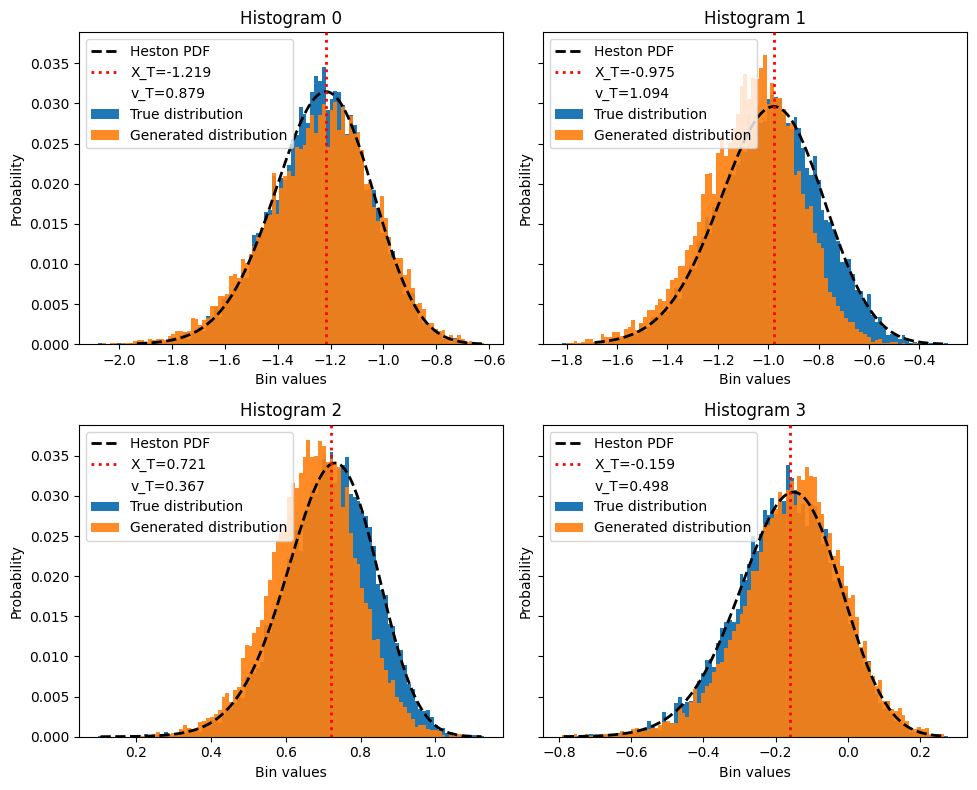
\includegraphics[scale=0.35]{images/srforgan_samples_2.png}
    \caption{Samples obtained using fixed $x_0$, $\mu$, $v_0$, $\theta$, $\kappa$, $\rho$ and $\sigma_v$}
\end{figure}
\end{frame}

\begin{frame}{SRForGAN -- Heston test with variable vol parameter}
  
\begin{figure}[H]
    \centering
    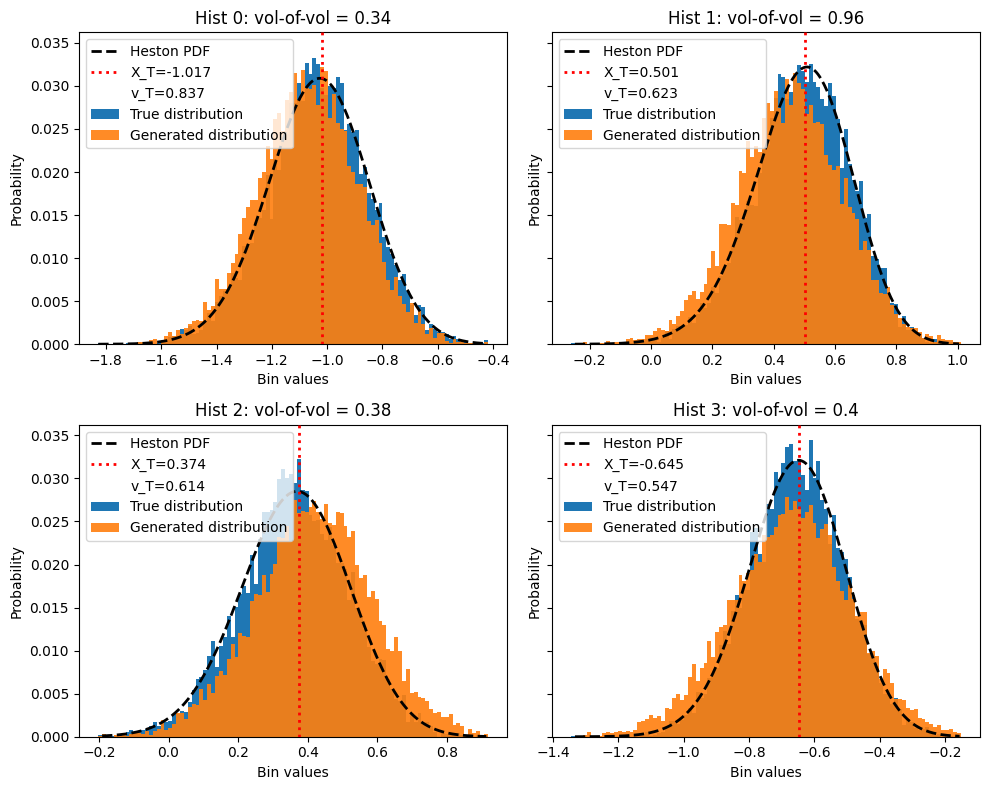
\includegraphics[scale=0.35]{images/srforgan_samples_volvol.png}
    \caption{Samples obtained using fixed $x_0$, $\mu$, $v_0$, $\theta$, $\kappa$, $\rho$ but different $\sigma_v$}
\end{figure}
\end{frame}

\begin{frame}{SRForGAN -- Heston test with variable parameters}
\begin{figure}[H]
    \centering
    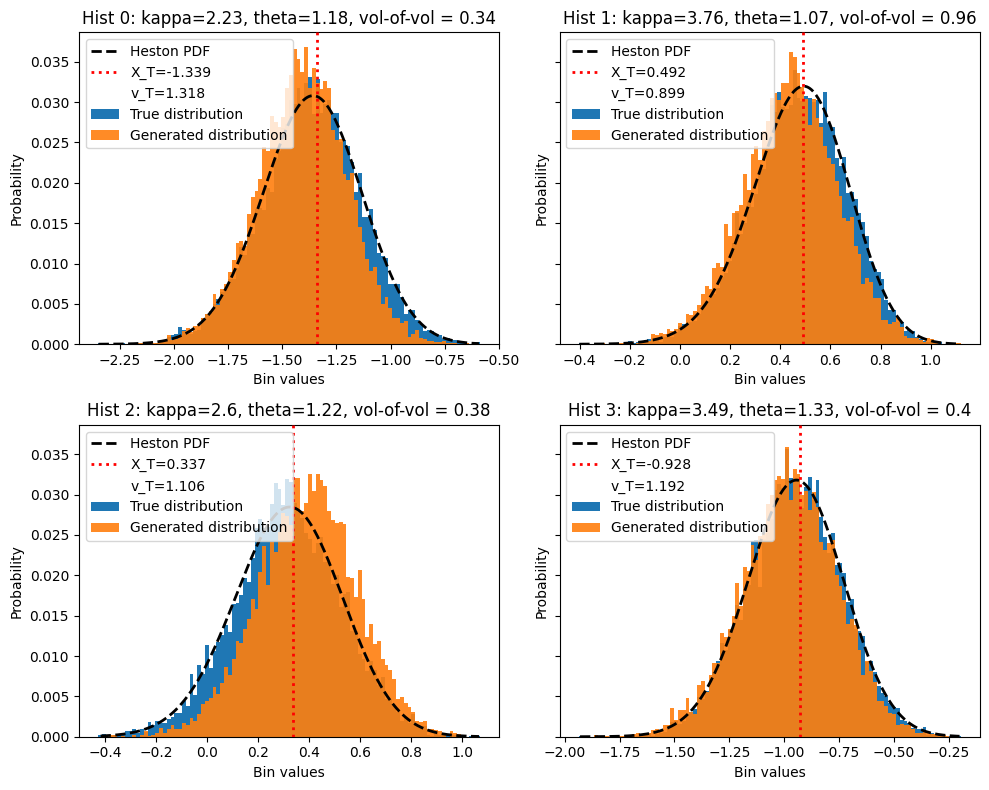
\includegraphics[scale=0.35]{images/srforgan_samples_all_params.png}
    \caption{Samples obtained using fixed $x_0$, $\mu$, $v_0$, but different $\theta$, $\kappa$, and $\sigma_v$}
\end{figure}
\end{frame}



\begin{frame}[plain]

\centering
\vfill

{\Huge \textbf{Thank You}}


\vfill

\end{frame}

